\documentclass[12pt, border=8pt]{standalone}
\usepackage{tikz}
\usepackage{amsmath, amssymb, bm}
\usepackage{xcolor}
\usepackage{booktabs}
\usetikzlibrary{positioning, arrows.meta, calc, fit, backgrounds, 3d}

\begin{document}


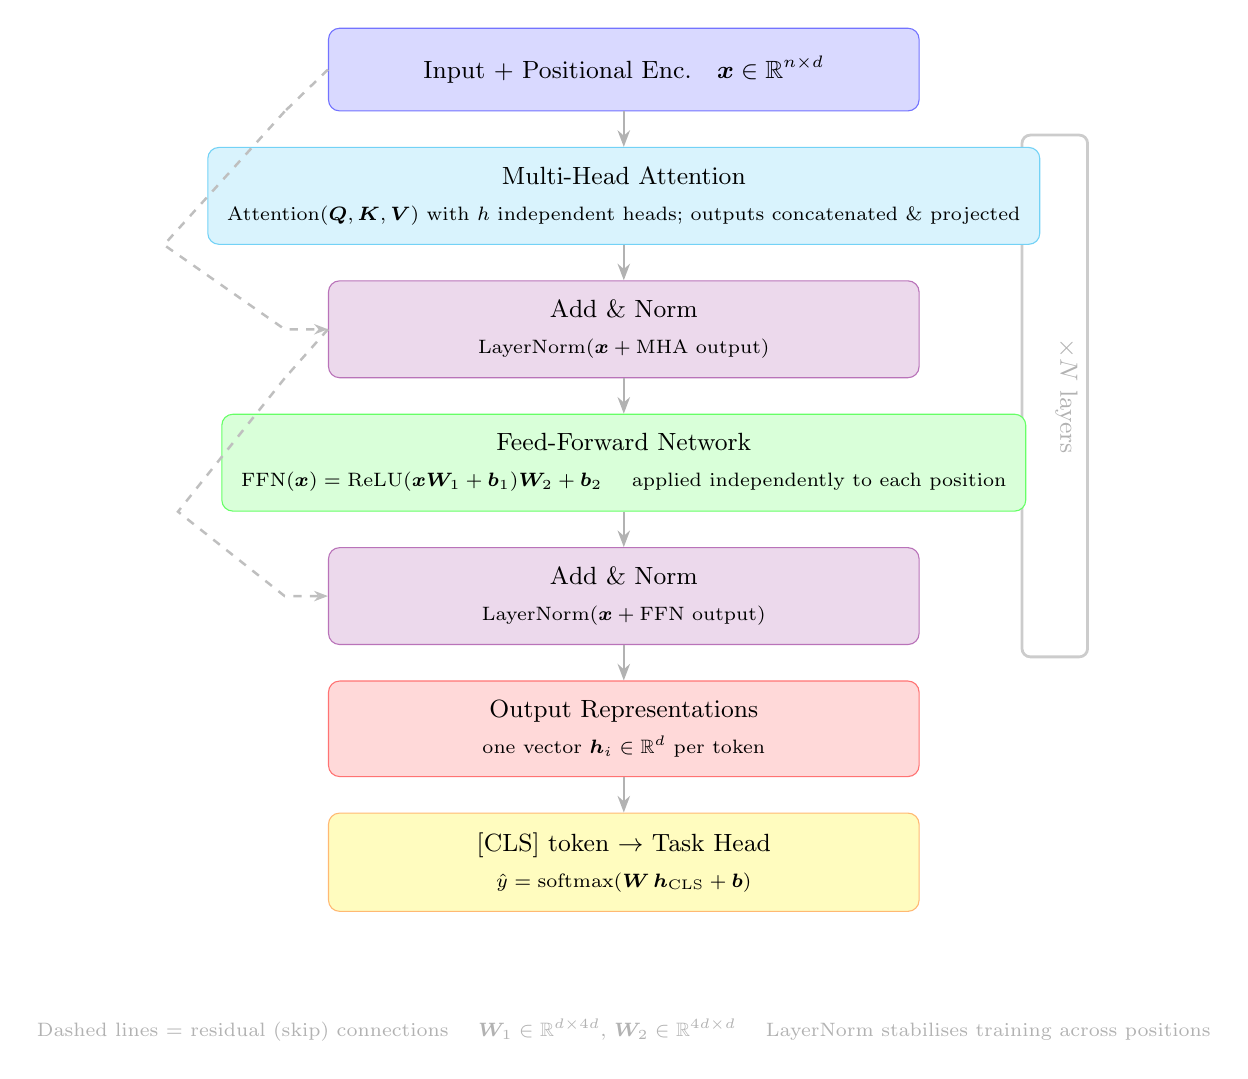
\begin{tikzpicture}[
  every node/.style={font=\small},
  arr/.style={-{Stealth[length=6pt]}, thick, gray!60},
  block/.style={draw, rounded corners=4pt, minimum width=7.5cm, minimum height=1.05cm,
                align=center, inner sep=7pt, font=\small},
  res/.style={dashed, gray!50, -{Stealth[length=5pt]}, line width=0.9pt}
]

% ---- Stack of blocks (bottom-to-top order, placed top-to-bottom) ----

\node[block, fill=blue!15, draw=blue!55] (input) at (0,0)
  {Input + Positional Enc.\quad $\bm{x} \in \mathbb{R}^{n \times d}$};

\node[block, fill=cyan!15, draw=cyan!55, below=0.45cm of input] (mha)
  {Multi-Head Attention\\[2pt]
   {\scriptsize $\text{Attention}(\bm{Q},\bm{K},\bm{V})$ with $h$ independent heads; outputs concatenated \& projected}};

\node[block, fill=violet!15, draw=violet!55, below=0.45cm of mha] (addnorm1)
  {Add \& Norm\\[2pt]
   {\scriptsize $\text{LayerNorm}(\bm{x} + \text{MHA output})$}};

\node[block, fill=green!15, draw=green!60, below=0.45cm of addnorm1] (ffn)
  {Feed-Forward Network\\[2pt]
   {\scriptsize $\text{FFN}(\bm{x}) = \text{ReLU}(\bm{x}\bm{W}_1 + \bm{b}_1)\bm{W}_2 + \bm{b}_2$
    \quad applied independently to each position}};

\node[block, fill=violet!15, draw=violet!55, below=0.45cm of ffn] (addnorm2)
  {Add \& Norm\\[2pt]
   {\scriptsize $\text{LayerNorm}(\bm{x} + \text{FFN output})$}};

\node[block, fill=red!15, draw=red!55, below=0.45cm of addnorm2] (outrepr)
  {Output Representations\\[2pt]
   {\scriptsize one vector $\bm{h}_i \in \mathbb{R}^d$ per token}};

\node[block, fill=yellow!25, draw=orange!55, below=0.45cm of outrepr] (cls)
  {{[CLS]} token $\to$ Task Head\\[2pt]
   {\scriptsize $\hat{y} = \text{softmax}(\bm{W}\,\bm{h}_{\text{CLS}} + \bm{b})$}};

% ---- Forward arrows ----
\draw[arr] (input.south) -- (mha.north);
\draw[arr] (mha.south) -- (addnorm1.north);
\draw[arr] (addnorm1.south) -- (ffn.north);
\draw[arr] (ffn.south) -- (addnorm2.north);
\draw[arr] (addnorm2.south) -- (outrepr.north);
\draw[arr] (outrepr.south) -- (cls.north);

% ---- Residual (skip) connections on left side ----
% Residual 1: input -> addnorm1
\draw[res]
  ($(input.south west) + (-0.55, 0)$) -- ($(mha.south west) + (-0.55, 0)$)
  node[midway, left, font=\tiny, text=gray!60] {}
  -- ($(addnorm1.west) + (-0.55, 0)$) -- (addnorm1.west);
\draw[res, -{}, >={Stealth}]
  ($(input.west) + (0,0)$) -- ($(input.south west) + (-0.55,0)$);

% Residual 2: addnorm1 -> addnorm2
\draw[res]
  ($(addnorm1.south west) + (-0.55,0)$) -- ($(ffn.south west) + (-0.55,0)$)
  -- ($(addnorm2.west) + (-0.55,0)$) -- (addnorm2.west);
\draw[res, -{}, >={Stealth}]
  ($(addnorm1.west)+(0,0)$) -- ($(addnorm1.south west)+(-0.55,0)$);

% ---- xN bracket on the right ----
\begin{scope}[on background layer]
  \draw[draw=gray!40, line width=1.0pt, rounded corners=3pt]
    ($(mha.north east) + (0.6, 0.15)$) rectangle ($(addnorm2.south east) + (1.3,-0.15)$);
\end{scope}
\node[font=\small, text=gray!60, rotate=-90] at
  ($(mha.north east)!0.5!(addnorm2.south east) + (1.1,0)$) {$\times N$ layers};

% ---- Footnote ----
\node[font=\scriptsize, text=gray!60, align=left] at (0, -12.2)
  {Dashed lines $=$ residual (skip) connections \quad
   $\bm{W}_1 \in \mathbb{R}^{d\times 4d}$, $\bm{W}_2 \in \mathbb{R}^{4d\times d}$ \quad
   LayerNorm stabilises training across positions};

\end{tikzpicture}

\end{document}
